% Template:     Informe LaTeX
% Documento:    Archivo principal
% Versión:      8.2.3 (03/04/2023)
% Codificación: UTF-8
%
% Autor: Pablo Pizarro R.
%        pablo@ppizarror.com
%
% Manual template: [https://latex.ppizarror.com/informe]
% Licencia MIT:    [https://opensource.org/licenses/MIT]

% CREACIÓN DEL DOCUMENTO
\documentclass[
	spanish, % Idioma: spanish, english, etc.
	letterpaper, oneside
]{article}

% INFORMACIÓN DEL DOCUMENTO
\def\documenttitle {\textbf{Laboratorio 1}}
\def\documentsubtitle {}
\def\documentsubject {}

\def\documentauthor {Daniel Minaya}
\def\coursename {\textbf{Modelos Generativos Profundos}}
\def\coursecode {\textbf{MDS7203}}

\def\universityname {Universidad de Chile}
\def\universityfaculty {Facultad de Ciencias Físicas y Matemáticas}
\def\universitydepartment {Departamento de Ingeniería Matemática}
\def\universitydepartmentimage {../Template_Informe/img/departamentos/dim}
\def\universitydepartmentimagecfg {height=1.57cm}
\def\universitylocation {Santiago de Chile}

% INTEGRANTES, PROFESORES Y FECHAS
\def\authortable {
	\begin{tabular}{ll}
		\textbf{Estudiante:}
		& \begin{tabular}[t]{l}
			Daniel Minaya
		\end{tabular} \\
		\textbf{Profesor:}
		& \begin{tabular}[t]{l}
			Felipe Tobar
		\end{tabular} \\
		\textbf{Auxiliares:}
		& \begin{tabular}[t]{l}
			Cristóbal Alcázar\\
			Camilo Carvajal
		\end{tabular} \\
		& \\
		\multicolumn{2}{l}{\textbf{Fecha de entrega:} 8 de septiembre}
	\end{tabular}
}

% IMPORTACIÓN DEL TEMPLATE
\input{../Template_Informe/template}

\newcommand\sol[1]{%
	{\color{Blue}{#1}}
}

\usepackage{paracol}
\usepackage{tikz}
\usetikzlibrary{arrows}

% INICIO DE PÁGINAS
\begin{document}

% PORTADA
\templatePortrait

% CONFIGURACIÓN DE PÁGINA Y ENCABEZADOS
\templatePagecfg

% RESUMEN O ABSTRACT
%\begin{abstractd}
%	\lipsum[1] % Párrafo ejemplo, se puede borrar
%\end{abstractd}

% TABLA DE CONTENIDOS - ÍNDICE
%\templateIndex

% CONFIGURACIONES FINALES
\templateFinalcfg

% ======================= INICIO DEL DOCUMENTO =======================

\section*{Parte 2 (Modelos gráficos)}
\begin{enumerate}
	\item[(a)] Sabemos que la cantidad de polen puede causar irritación en nariz y ojos en algunos casos, por lo que habría una dependencia entre estas dos variables. Además, la cantidad de polen también afecta a la probabilidad de sufrir Rinitis alérgica, por lo que tendríamos otra dependencia. También es sabido que si se tiene Rinitis alérgica, entonces es probable tener irritación en nariz y ojos. Por último, suponiendo que la variable de tener un familiar con Rinitis alérgica hace referencia a una enfermedad hereditaria, y no a una enfermedad que pueda ser contagiada, tendríamos que esta variable aumentaría las posibilidades de tener la Rinitas alérgica.

	Definiendo las variables aleatorias \(I=\) ``Tener irritación en nariz y ojos'', \(P=\) ``cantidad de polen en el ambiente'', \(R=\) ``Tener Rinitis alérgica'' y \(F=\) ``Tener un familiar con Rinitis alérgica'', entonces, por todo lo anterior, el modelo gráfico que representa el problema estaría dado por el siguiente DAG:

\begin{center}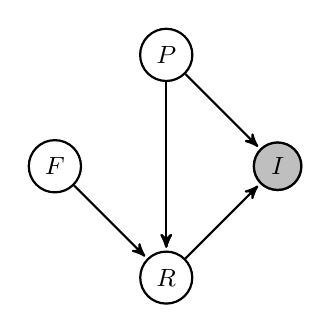
\begin{tikzpicture}[->,>=stealth',shorten >=1pt,auto,node distance=2cm,
	thick,main node/.style={circle,draw,font=\sffamily\small\bfseries}]
	
	\node[main node] (1) {\(P\)};
	\node[main node] (2) [below left of=1] {\(F\)};
	\node[main node] (3) [below right of=2] {\(R\)};
	\node[main node, preaction={fill=gray}, opacity=0.5] (5) [below right of=1] {\color{white}{\(I\)}};
	\node[main node] (4) [below right of=1] {\(I\)};
	
	\path[every node/.style={font=\sffamily\small}]
	(1) edge node [left] {} (4)
	(1) edge node [left] {} (3)
	(1) edge node [left] {} (3)
	(2) edge node [left] {} (3)
	(3) edge node [left] {} (4);
\end{tikzpicture}\end{center}

\item[(b)] Usando la notación anterior, queremos encontrar \(\P(R|I)\). Según el modelo gráfico planteado, la probabilidad conjunta está dada por:\[\P(P,I,F,R)=\P(P)\cdot\P(F)\cdot\P(R|F,P)\cdot\P(I|R,P),\]
donde todas las probabilidades en el lado izquierdo son conocidas a priori. De este modo, por el teorema de Bayes tenemos:\[\P(R|I)=\frac{\P(I|R)\P(R)}{\P(I)},\]
luego, por el teorema de probabilidades tenemos:\begin{align*}
	\P(I|R)&=\sum_{k}\P(I|R,P=k)\P(P=k),\\
	\P(R)&=\sum_{k}\sum_{j}\P(R|F=j,P=k)\P(F=j)\P(P=k),\\
	\P(I)&=\sum_{k}\sum_{j}\P(I|R=j,P=k)\P(R=j)\P(P=k),
\end{align*}
donde las primeras dos igualdades están en términos de probabilidades conocidas, mientras que la última igualdad tiene el término \(\P(R=j)\) que se conoce de la segunda igualdad, por lo que \(\P(R|I)\) se obtendría calculando las probabilidades respectivas.

\item[(c)] En este caso debemos agregar una nueva variable al modelo gráfico, llamemósla \(T=\) ``Test positivo''. Esta variable solo afecta a la probabilidad de tener Rinitis alérgica, por lo que el nuevo modelo gráfico estaría dado por:
\begin{center}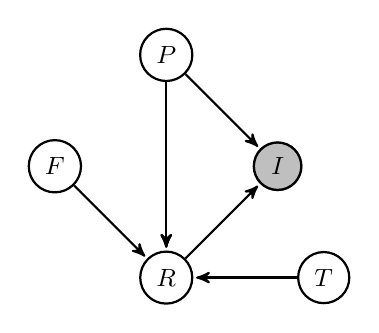
\begin{tikzpicture}[->,>=stealth',shorten >=1pt,auto,node distance=2cm,
		thick,main node/.style={circle,draw,font=\sffamily\small\bfseries}]
		
		\node[main node] (1) {\(P\)};
		\node[main node] (2) [below left of=1] {\(F\)};
		\node[main node] (3) [below right of=2] {\(R\)};
		\node[main node, preaction={fill=gray}, opacity=0.5] (5) [below right of=1] {\color{white}{\(I\)}};
		\node[main node] (4) [below right of=1] {\(I\)};
		\node[main node] (6) [right of=3] {\(T\)};
		
		\path[every node/.style={font=\sffamily\small}]
		(1) edge node [left] {} (4)
		(1) edge node [left] {} (3)
		(1) edge node [left] {} (3)
		(2) edge node [left] {} (3)
		(6) edge node [left] {} (3)
		(3) edge node [left] {} (4);
\end{tikzpicture}\end{center}
Con este nuevo modelo gráfico, la nueva probabilidad conjunto sería:
\[\P(P,I,F,R,T)=\P(P)\cdot\P(F)\cdot\P(T)\cdot\P(R|F,P,T)\P(I|R,P),\]
luego la probabilidad \(\P(R|I)=\frac{\P(I|R)\P(R)}{\P(I)}\) solo vería afectada su término \(\P(R)\), el cual ahora estaría dado por
\begin{align*}
	\P(R)&=\sum_{k}\sum_{j}\sum_i\P(R|T=i,F=j,P=k)\P(T=i)\P(F=j)\P(P=k).
\end{align*}
Notar que esto afectaría indirectamente a \(\P(I)\) también, pues depende de \(\P(R)\).

\item[(d)] En este caso utilizamos \(P\) como variable continua que sigue una distribución semi-normal, pues al tratarse de la cantidad de polen en el ambiente, ésta puede tomar solo valores positivos. En este caso, la expresión para \(\P(R|I)\) cambia, pues pasamos \(P\) de una variable discreta a una continua, por lo que:
\begin{align*}
	\P(I|R)&=\int_0^\infty\P(I|R,P=x)f_P(x)dx,\\
	\P(R)&=\int_0^\infty\sum_{j}\sum_i\P(R|T=i,F=j,P=x)\P(T=i)\P(F=j)f_P(x)dx,\\
	\P(I)&=\int_0^\infty\sum_{j}\P(I|R=j,P=x)\P(R=j)f_P(x)dx,
\end{align*}
donde \(f_P(x)\) es la densidad de una semi-normal, es decir, \(f_P(x)=\sqrt{\frac{2}{\sigma^2\pi}}e^{-x^2/2\sigma^2}\).

\item[(e)] Definamos \(X_t=\) ``cantidad de polen en el tiempo \(t\)'' e \(Y_t=\) ``irritación en nariz y ojos en el tiempo \(t\)'' procesos aleatorios. Como suponemos que el futuro es independiente del paso condicionado al presente, entonces \((X_t)_t\) es una cadena de Markov, por lo que nuestro modelo gráfico ahora es un Hidden Markov Model representado por:

\begin{center}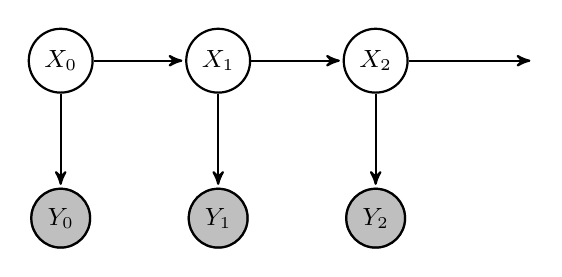
\begin{tikzpicture}[->,>=stealth',shorten >=1pt,auto,node distance=2cm,
		thick,main node/.style={circle,draw,font=\sffamily\small\bfseries}]
		
		\node[main node] (1) {\(X_0\)};
		\node[main node] (2) [right of=1] {\(X_1\)};
		\node[main node] (3) [right of=2] {\(X_2\)};
		\coordinate[right of=3] (4);
		\node[main node, preaction={fill=gray}, opacity=0.5] (8) [below of=1] {\color{white}{\(Y_0\)}};
		\node[main node] (5) [below of=1] {\(Y_0\)};
		\node[main node, preaction={fill=gray}, opacity=0.5] (8) [below of=2] {\color{white}{\(Y_1\)}};
		\node[main node] (6) [below of=2] {\(Y_1\)};
		\node[main node, preaction={fill=gray}, opacity=0.5] (8) [below of=3] {\color{white}{\(Y_2\)}};
		\node[main node] (7) [below of=3] {\(Y_2\)};
		
		\path[every node/.style={font=\sffamily\small}]
		(1) edge node [left] {} (2)
		(2) edge node [left] {} (3)
		(3) edge node [left] {} (4)
		(1) edge node [left] {} (5)
		(2) edge node [left] {} (6)
		(3) edge node [left] {} (7);
\end{tikzpicture}\end{center}

Queremos predecir la cantidad de polen cada 30 minutos usando como única medición el nivel de irritación en nariz y ojos, es decir, se quiere calcular \(\P(X_{30t}|Y_{1:30t})=\P(X_{30t}|Y_1,\ldots,Y_{30t})\), para lo cual se podría utilizar el filtro de Kalman.
\end{enumerate}

\section*{Parte 3 (Introducción al Transporte Óptimo)}
\begin{enumerate}
\item[(a)] Dadas dos distribuciones discretas \(\alpha=\sum_{i=1}^na_i\delta_{x_i}\) y \(\beta=\sum_{j=1}^mb_j\delta_{y_j}\). El transporte óptimo entre \(\alpha\) y \(\beta\) está dado por \(P^\ast\) que resuelve el siguiente problema de minimización:
\begin{equation}\tag{\(P\)}
	\begin{aligned}
			\min_{P\in\mathcal M_{nm}} \quad & \sum_{i=1}^n\sum_{j=1}^m P_{ij}C_{ij}\\
			\textrm{s.a.} \quad & \sum_{j=1}^mP_{ij} = a_i,~\forall i\in[n] \\
			& \sum_{i=1}^nP_{ij} = b_j,~\forall j\in[m]\\
			& P_{ij}\geq0,~\forall i\in[n],j\in[m]
		\end{aligned}
\end{equation}
donde \(C_{ij}=\|x_i-y_j\|^2\). Identificando las matrices \(P\) y \(C\) como vectores en \(\R^{nm}\) apilando las filas de la siguiente manera:

\[P_{i\bullet}^T=\begin{pmatrix}P_{i1}\\\vdots\\P_{im}\end{pmatrix}\in\R^m\Rightarrow P=\begin{pmatrix}
		P_{1\bullet}^T\\
		\hline
		\vdots\\
		\hline
		P_{n\bullet}^T
	\end{pmatrix}\in\R^{nm},\quad C_{i\bullet}^T=\begin{pmatrix}C_{i1}\\\vdots\\C_{im}\end{pmatrix}\in\R^m\Rightarrow C=\begin{pmatrix}
	C_{1\bullet}^T\\
	\hline
	\vdots\\
	\hline
	C_{n\bullet}^T
	\end{pmatrix}\in\R^{nm},\]
	
	el problema \((P)\) se puede reescribir como el siguiente problema lineal \((PL)\):
	\begin{equation}\tag{\(PL\)}
		\begin{aligned}
				\min_{P\in\R^{nm}} \quad & C^TP\\
				\textrm{s.a.} \quad & ZP=\omega\\
				& P\geq0
			\end{aligned}
	\end{equation}
	donde usamos
	\begin{equation*}
		Z=\left[\begin{array}{ c | c | c}
				A_1 & \cdots & A_n \\
				\hline
				I_m & \cdots & I_m
			\end{array}\right]\in\mathcal M_{n+m,nm},\quad\omega=\begin{pmatrix}a_1&\cdots&a_n&\vline  &b_1&\cdots &b_m\end{pmatrix}^T\in\R^{n+m}
	\end{equation*}
	y \(A_i\in\mathcal M_{nm}\) es una matriz de \(0\)'s en todas las posiciones excepto en la fila \(i\), que tiene solo \(1\)'s e \(I_m\) es la matriz identidad en \(\mathcal M_{mm}\).
	
	\item[(b)] Para el caso $d=1$ tenemos que $\Sigma_1=\sigma_1^2$ y $\Sigma_2=\sigma_2^2$ corresponden a las varianzas y $A=\sigma_1^{-1}\left(\sigma_1\sigma_2^2\sigma_1\right)^{1/2}\sigma_1^{-1}=\frac{\sigma_2}{\sigma_1}$, por lo cual el transporte óptimo viene dado por 
	
	$$T(x)=\mu_2+\frac{\sigma_2}{\sigma_1}(x-\mu_1).$$
	
	Notemos que el transporte óptimo se puede ver como tres transformaciones que llevan $\mathcal N(\mu_1,\Sigma_1)$ a $\mathcal N(\mu_2,\Sigma_2)$. Sea $x\in\mathcal N(\mu_1,\sigma_1^2)$, entonces $x-\mu_1\in\mathcal N(0,\sigma_1)$, es decir, llevamos $x$ al origen, luego al multiplicar por $A$ tenemos $A(x-\mu_1)\in\mathcal N(0,\sigma_2^2)$, es decir, achicamos por $\sigma_1$ y amplificamos por $\sigma_2$, y por último, trasladamos a la segunda distribución de modo que $\mu_2+A(x-\mu_1)\in\mathcal N(\mu_2,\sigma_2^2)$.
	
	De manera general (para $d>1$) la intución es la misma, primero trasladamos los datos al origen, luego en el origen deformamos la primera distribución hasta obtener la forma de la segunda distribución. Por último, una vez obtenemos la forma correcta, centramos en la media de la distribución objetivo.
	
	\item[(c)] Sampleamos muestras de dos distribuciones normales. Nuestra distribución inicial será \(\mathcal N(0,3)\) y samplearemos \(50\) muestras, y la distribución objetivo será \(\mathcal N(5,2)\) y samplearemos \(60\) muestras.
	
	\begin{figure}[H]
		\subfloat{\includegraphics[scale=0.6]{Imágenes/distributions-1d.pdf}}
		\caption{Muestras de distribuciones normales.}
	\end{figure}
	
	Aplicando el método anterior, obtenemos el siguiente transporte óptimo.
	
	\begin{figure}[H]
		\subfloat{\includegraphics[scale=0.5]{Imágenes/ot-1d.pdf}}
		\caption{Matriz de distancias y transporte óptimo.}
	\end{figure}
	
	El valor óptimo obtenido por el método fue de \(22.88\), mientras que la distancia de Wasserstein entre las dos distribuciones es \(25.10\), por lo que obtuvimos un resultado parecido usando el método que estaba aproximando una normal mediante muestras.
	
	\item[(d)] Sampleamos muestras de dos distribuciones normales en \(\R^2\). La distribución inicial será \(\mathcal N(\mu_1,\Sigma_1)\) de la cual samplearemos \(10\) muestras, y la distribución objetivo será \(\mathcal N(\mu_2,\Sigma_2)\) de la cual samplearemos \(15\) muestras, donde\[\mu_1=\begin{pmatrix}
		0\\0
	\end{pmatrix},\quad\mu_2=\begin{pmatrix}
	10\\3
\end{pmatrix},\quad\Sigma_1=\begin{pmatrix}
1&0\\0&1
\end{pmatrix},\quad\Sigma_2=\begin{pmatrix}
2&1\\1&2
\end{pmatrix}\]
son las medias y matrices de covarianza respectivas.
	
	\begin{figure}[H]
		\subfloat{\includegraphics[scale=0.6]{Imágenes/samples-2d.pdf}}
		\caption{Muestras de distribuciones normales en \(\R^2\)}
	\end{figure}
	
	Obtenemos el siguiente transporte óptimo.
	
	\begin{figure}[H]
		\subfloat{\includegraphics[scale=0.5]{Imágenes/ot-2d.pdf}}
		\caption{Matriz de distancias y transporte óptimo.}
	\end{figure}
	
	Esto se traduce en las siguientes asignaciones.
	
	\begin{figure}[H]
		\subfloat{\includegraphics[scale=0.55]{Imágenes/asignations.pdf}}
		\caption{Asignaciones.}
	\end{figure}
	
	\item[(e)] El baricentro nos permite visualizar cómo ocurre la transformación de la distribución inicial hacia la distribución objetivo.
	
	\begin{multicols}{2}
	\begin{figure}[H]
		\subfloat{\includegraphics[width=\linewidth, height=0.6\linewidth]{Imágenes/barycenter_0.00}}\\
		\subfloat{\includegraphics[width=\linewidth, height=0.6\linewidth]{Imágenes/barycenter_0.76}}
	\end{figure}
	\begin{figure}[H]
		\subfloat{\includegraphics[width=\linewidth, height=0.6\linewidth]{Imágenes/barycenter_0.33}}\\
		\subfloat{\includegraphics[width=\linewidth, height=0.6\linewidth]{Imágenes/barycenter_1.00}}
	\end{figure}
	\end{multicols}

En el siguiente \href{https://github.com/DanielMinaya1/MDS7203/blob/main/Laboratorio_1/barycenter.gif}{link} se puede ver una animación para \(100\) valores de \(t\) entre \(0\) y \(1\).
\end{enumerate}
% FIN DEL DOCUMENTO
\end{document}